%%%%%%%%%%%%%%%%%%%%%%%%%%%%%%%%%%%%%%%%%
% baposter Landscape Poster
% LaTeX Template
% Version 1.0 (11/06/13)
%
% baposter Class Created by:
% Brian Amberg (baposter@brian-amberg.de)
%
% This template has been downloaded from:
% http://www.LaTeXTemplates.com
%
% License:
% CC BY-NC-SA 3.0 (http://creativecommons.org/licenses/by-nc-sa/3.0/)
%
%%%%%%%%%%%%%%%%%%%%%%%%%%%%%%%%%%%%%%%%%

%----------------------------------------------------------------------------------------
%	PACKAGES AND OTHER DOCUMENT CONFIGURATIONS
%----------------------------------------------------------------------------------------

\documentclass[landscape,a0paper,fontscale=0.285]{baposter} % Adjust the font scale/size here

\usepackage{graphicx} % Required for including images
\graphicspath{{figures/}} % Directory in which figures are stored

\usepackage{amsmath} % For typesetting math
\usepackage{amssymb} % Adds new symbols to be used in math mode

\usepackage{booktabs} % Top and bottom rules for tables
\usepackage{enumitem} % Used to reduce itemize/enumerate spacing
\usepackage{palatino} % Use the Palatino font
\usepackage[font=small,labelfont=bf]{caption} % Required for specifying captions to tables and figures

\usepackage{multicol} % Required for multiple columns
\usepackage{multirow}
\setlength{\columnsep}{1.5em} % Slightly increase the space between columns
\setlength{\columnseprule}{0mm} % No horizontal rule between columns

\usepackage{tikz} % Required for flow chart
\usetikzlibrary{shapes,arrows} % Tikz libraries required for the flow chart in the template

\newcommand{\compresslist}{ % Define a command to reduce spacing within itemize/enumerate environments, this is used right after \begin{itemize} or \begin{enumerate}
\setlength{\itemsep}{1pt}
\setlength{\parskip}{0pt}
\setlength{\parsep}{0pt}
}

\definecolor{lightblue}{rgb}{0.145,0.6666,1} % Defines the color used for content box headers

\begin{document}

\begin{poster}
{
headerborder=closed, % Adds a border around the header of content boxes
colspacing=1em, % Column spacing
bgColorOne=white, % Background color for the gradient on the left side of the poster
bgColorTwo=white, % Background color for the gradient on the right side of the poster
borderColor=lightblue, % Border color
headerColorOne=black, % Background color for the header in the content boxes (left side)
headerColorTwo=lightblue, % Background color for the header in the content boxes (right side)
headerFontColor=white, % Text color for the header text in the content boxes
boxColorOne=white, % Background color of the content boxes
textborder=roundedleft, % Format of the border around content boxes, can be: none, bars, coils, triangles, rectangle, rounded, roundedsmall, roundedright or faded
eyecatcher=true, % Set to false for ignoring the left logo in the title and move the title left
headerheight=0.1\textheight, % Height of the header
headershape=roundedright, % Specify the rounded corner in the content box headers, can be: rectangle, small-rounded, roundedright, roundedleft or rounded
headerfont=\Large\bf\textsc, % Large, bold and sans serif font in the headers of content boxes
%textfont={\setlength{\parindent}{1.5em}}, % Uncomment for paragraph indentation
linewidth=2pt % Width of the border lines around content boxes
}
%----------------------------------------------------------------------------------------
%	TITLE SECTION 
%----------------------------------------------------------------------------------------
%
{
\includegraphics[height=4em]{upc.png}} % logo on the left
{\bf\textsc{Stroke Prediction via Supervised Methods}\vspace{0.5em}}
{\textsc{Arnau Abella and Antoni Casas \hspace{12pt} Universitat Polit\`ecnica de Catalunya}}
{
\includegraphics[height=4em]{upc.png}} % logo on the right

%----------------------------------------------------------------------------------------
%	INTRODUCTION
%----------------------------------------------------------------------------------------

\headerbox{Introduction}{name=introduction,column=0,span=2,row=0}{
  Strokes are an unexpected \textbf{killer} and \textbf{hard to predict}, being the second leading cause of death globally. Therefore, the detection of segments of the population at risk could enhance the ability of hospitals and other medical teams to offer early treatments and screenings to reduce this risk. \\

  Our goal is to \textbf{predict whether or not an individual is going to suffer a stroke}.
}

%----------------------------------------------------------------------------------------
%	RESULTS 1
%----------------------------------------------------------------------------------------

\headerbox{Preliminary Results}{name=results,column=2,span=2,row=0}{
\begin{center}
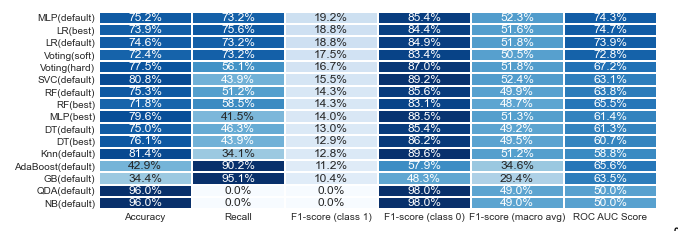
\includegraphics[width=0.9\linewidth]{Results-Table.png}
\captionof{figure}{Validation scores after hyperparameters tunning}
\label{fig:results}
\end{center}

The results show that the best models are the ones with \textbf{higher regularization}. It seems that the issue is \textbf{severe overfitting} due to the data imbalance and the scarcity of data. In our case, the models which achieved the best results were the multi-layer perceptron, the logistic regression with $l_{2}$-penalty and the voting classifier. Finally, after hyper-parameter tunning, we have chosen the \textbf{logistic regression} which achieves the highest f1-score and recall among the bests.
}

%----------------------------------------------------------------------------------------
%	REFERENCES
%----------------------------------------------------------------------------------------

\headerbox{References}{name=references,column=0,above=bottom}{

\renewcommand{\section}[2]{\vskip 0.05em} % Get rid of the default "References" section title
\nocite{*} % Insert publications even if they are not cited in the poster
\small{ % Reduce the font size in this block
\bibliographystyle{unsrt}
\bibliography{poster}
}}

%----------------------------------------------------------------------------------------
%	FUTURE RESEARCH
%----------------------------------------------------------------------------------------

\headerbox{Future Research}{name=futureresearch,column=1,span=2,aligned=references,above=bottom}{ % This block is as tall as the references block

\begin{multicols}{2}
  The data seems \textbf{too poor} to be able to create a good model for the minority class, however, it might be possible that there exists a transformation where, in the new space, the data is good enough to generalize with the current data. \\ Ignoring such event, the only possible work is expanding the data, via new variables recorded, or by \textbf{adding more samples}.

\end{multicols}
}

%----------------------------------------------------------------------------------------
%	CONTACT INFORMATION
%----------------------------------------------------------------------------------------

\headerbox{Contact Information}{name=contact,column=3,aligned=references,above=bottom}{ % This block is as tall as the references block

\begin{description}\compresslist
\item[Web] github.com/monadplus/ml-project
\item[Email] arnauabella@gmail.com
\item[Phone] +34 618 459 006
\end{description}
}

%----------------------------------------------------------------------------------------
%	CONCLUSION
%----------------------------------------------------------------------------------------

\headerbox{Conclusion}{name=conclusion,column=2,span=2,row=0,below=results,above=references}{

\begin{multicols}{2}

  \begin{center}
  \includegraphics[width=0.9\linewidth]{rocfinak.png}
  \captionof{figure}{ROC Curve on Test Data}
  \label{fig:roc}
  \end{center}

  Out of all our models, the ones most robust to overfitting were the ones who managed to perform well on the minority class. We believe this to be a case of a lack of data, since certain spaces of the hyperplane are left either unpopulated or with so little population that boundaries cannot be established properly, leading to overfitting and poor generalization.\\

  Our best model was the Logistic Regression with $L_{2}$ loss, a simple linear method, but extremely hard to overfit, with an interesting ROC curve, which could be exploited to obtain the best balance between false positives and true positives, since the focus is on achieving the highest number of true positives on the minority class, since a misdiagnosis can be fatal.\\

  % We can also see that of all the variables, those with the highest effect on stroke are, first of all and by far, age, then far behind average glucose level and bmi, with the rest of variables trailing behind. These relations might help understand strokes better.

\end{multicols}
}

%----------------------------------------------------------------------------------------
%	MATERIALS AND METHODS
%----------------------------------------------------------------------------------------

\headerbox{Materials \& Methods}{name=method,column=0,below=introduction,bottomaligned=conclusion}{ % This block's bottom aligns with the bottom of the conclusion block

  The stroke prediction dataset is composed by \textbf{11 features}: $3$ numerical and $8$ categorical. The dataset only has \textbf{5110 observations}. The binary classification problem is \textbf{highly imbalanced}, with only a $5\%$ of the population belonging to the positive class.\\

  To deal with the imbalance, we applied \textbf{SMOTE} which applies the over-sampling method \emph{SMOTE} combined with the under-sampling method \emph{Tomek Links}. The combination of both should re-balance the dataset while avoiding the creation of noisy samples from the interpolation of outliers and inliers.\\

  We have also explored \textbf{factor analysis}, in particular MCA, and dimensionality.\\

  We considered the following models:

\begin{itemize}\compresslist
\item Logistic Regression with Regularization
\item Bayesian Models
\item Support Vector Machines
\item Decision Trees
\item Ensemble Methods: Random Forest, Ada Boosting, and Voting Classifiers
\item Neural Networks
\end{itemize}

  We focused on achieving the best \emph{F1-score} while keeping a high \emph{recall}.
}

%----------------------------------------------------------------------------------------
%	RESULTS 2
%----------------------------------------------------------------------------------------

\headerbox{Final Results}{name=results2,column=1,below=introduction,bottomaligned=conclusion}{ % This block's bottom aligns with the bottom of the conclusion block

We evaluate how our best model \emph{generalises} using the test data. Our optimized model achieves a \textbf{$79\%$ of true positives on the minority class} which seems to be an accurate representation of its generalization capability.

\begin{center}
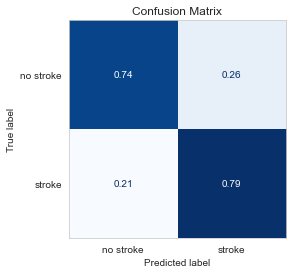
\includegraphics[width=.7\linewidth]{LogRedResult.png}
\captionof{figure}{Confusion Matrix on Test Data}
\end{center}

We can also see on the ROC curve (figure \ref{fig:roc}) that this model has an interesting quirk, and that's it that we \textbf{can achieve a true positive rate of 100\% on the minority class} if we also have a false positive rate of $60\%$ in the minority class, which means we can effectively never miss a possible stroke if we are willing to also deal with all the positives.

}

%----------------------------------------------------------------------------------------

\end{poster}

\end{document}
